\documentclass[12pt,a4paper]{article}
\title{Lab9-OpenCV}
\usepackage{ctex}
\usepackage{amsmath,amscd,amsbsy,amssymb,latexsym,url,bm,amsthm}
\usepackage{epsfig,graphicx,subfigure}
\usepackage{enumitem,balance}
\usepackage{wrapfig}
\usepackage{mathrsfs,euscript}
\usepackage[usenames]{xcolor}
\usepackage{hyperref}
\usepackage[vlined,ruled,commentsnumbered,linesnumbered]{algorithm2e}
\usepackage{float}
\usepackage{geometry}
\usepackage{listings}
\geometry{a4paper,scale=0.8}
\usepackage[T1]{fontenc}
\usepackage[utf8]{inputenc}
\usepackage{amssymb}
\usepackage{graphicx}
\usepackage{subfigure}
% --- Python code template ---
\usepackage[utf8]{inputenc}
% Default fixed font does not support bold face
\DeclareFixedFont{\ttb}{T1}{txtt}{bx}{n}{12} % for bold
\DeclareFixedFont{\ttm}{T1}{txtt}{m}{n}{12}  % for normal

% Custom colors
\usepackage{color}
\definecolor{deepblue}{rgb}{0,0,0.5}
\definecolor{deepred}{rgb}{0.6,0,0}
\definecolor{deepgreen}{rgb}{0,0.5,0}

\usepackage{listings}

% Python style for highlighting
\newcommand\pythonstyle{\lstset{
language=Python,
basicstyle=\ttm,
morekeywords={self},              % Add keywords here
keywordstyle=\ttb\color{deepblue},
emph={MyClass,__init__},          % Custom highlighting
emphstyle=\ttb\color{deepred},    % Custom highlighting style
stringstyle=\color{deepgreen},
frame=tb,                         % Any extra options here
showstringspaces=false
}}
% Python environment
\lstnewenvironment{python}[1][]
{
\pythonstyle
\lstset{#1}
}
{}

% Python for external files
\newcommand\pythonexternal[2][]{{
\pythonstyle
\lstinputlisting[#1]{#2}}}

% Python for inline
\newcommand\pythoninline[1]{{\pythonstyle\lstinline!#1!}}

% --- Python code template ---


% --- HTML lstlisting template --- %
\makeatletter
\usepackage{color}
\definecolor{lightgray}{rgb}{0.95, 0.95, 0.95}
\definecolor{darkgray}{rgb}{0.4, 0.4, 0.4}
%\definecolor{purple}{rgb}{0.65, 0.12, 0.82}
\definecolor{editorGray}{rgb}{0.95, 0.95, 0.95}
\definecolor{editorOcher}{rgb}{1, 0.5, 0} % #FF7F00 -> rgb(239, 169, 0)
\definecolor{editorGreen}{rgb}{0, 0.5, 0} % #007C00 -> rgb(0, 124, 0)
\definecolor{orange}{rgb}{1,0.45,0.13}		
\definecolor{olive}{rgb}{0.17,0.59,0.20}
\definecolor{brown}{rgb}{0.69,0.31,0.31}
\definecolor{purple}{rgb}{0.38,0.18,0.81}
\definecolor{lightblue}{rgb}{0.1,0.57,0.7}
\definecolor{lightred}{rgb}{1,0.4,0.5}
\usepackage{upquote}
\usepackage{listings}
% CSS
\lstdefinelanguage{CSS}{
  keywords={color,background-image:,margin,padding,font,weight,display,position,top,left,right,bottom,list,style,border,size,white,space,min,width, transition:, transform:, transition-property, transition-duration, transition-timing-function},	
  sensitive=true,
  morecomment=[l]{//},
  morecomment=[s]{/*}{*/},
  morestring=[b]',
  morestring=[b]",
  alsoletter={:},
  alsodigit={-}
}

% JavaScript
\lstdefinelanguage{JavaScript}{
  morekeywords={typeof, new, true, false, catch, function, return, null, catch, switch, var, if, in, while, do, else, case, break},
  morecomment=[s]{/*}{*/},
  morecomment=[l]//,
  morestring=[b]",
  morestring=[b]'
}

\lstdefinelanguage{HTML5}{
  language=html,
  sensitive=true,	
  alsoletter={<>=-},	
  morecomment=[s]{<!-}{-->},
  tag=[s],
  otherkeywords={
  % General
  >,
  % Standard tags
	<!DOCTYPE,
  </html, <html, <head, <title, </title, <style, </style, <link, </head, <meta, />,
	% body
	</body, <body,
	% Divs
	</div, <div, </div>, 
	% Paragraphs
	</p, <p, </p>,
	% scripts
	</script, <script,
  % More tags...
  <canvas, /canvas>, <svg, <rect, <animateTransform, </rect>, </svg>, <video, <source, <iframe, </iframe>, </video>, <image, </image>, <header, </header, <article, </article
  },
  ndkeywords={
  % General
  =,
  % HTML attributes
  charset=, src=, id=, width=, height=, style=, type=, rel=, href=,
  % SVG attributes
  fill=, attributeName=, begin=, dur=, from=, to=, poster=, controls=, x=, y=, repeatCount=, xlink:href=,
  % properties
  margin:, padding:, background-image:, border:, top:, left:, position:, width:, height:, margin-top:, margin-bottom:, font-size:, line-height:,
	% CSS3 properties
  transform:, -moz-transform:, -webkit-transform:,
  animation:, -webkit-animation:,
  transition:,  transition-duration:, transition-property:, transition-timing-function:,
  }
}

\lstdefinestyle{htmlcssjs} {%
  % General design
%  backgroundcolor=\color{editorGray},
  basicstyle={\footnotesize\ttfamily},   
  frame=b,
  % line-numbers
  xleftmargin={0.75cm},
  numbers=left,
  stepnumber=1,
  firstnumber=1,
  numberfirstline=true,	
  % Code design
  identifierstyle=\color{black},
  keywordstyle=\color{blue}\bfseries,
  ndkeywordstyle=\color{editorGreen}\bfseries,
  stringstyle=\color{editorOcher}\ttfamily,
  commentstyle=\color{brown}\ttfamily,
  % Code
  language=HTML5,
  alsolanguage=JavaScript,
  alsodigit={.:;},	
  tabsize=2,
  showtabs=false,
  showspaces=false,
  showstringspaces=false,
  extendedchars=true,
  breaklines=true,
  % German umlauts
  literate=%
  {Ö}{{\"O}}1
  {Ä}{{\"A}}1
  {Ü}{{\"U}}1
  {ß}{{\ss}}1
  {ü}{{\"u}}1
  {ä}{{\"a}}1
  {ö}{{\"o}}1
}
%
\lstdefinestyle{py} {%
language=python,
literate=%
*{0}{{{\color{lightred}0}}}1
{1}{{{\color{lightred}1}}}1
{2}{{{\color{lightred}2}}}1
{3}{{{\color{lightred}3}}}1
{4}{{{\color{lightred}4}}}1
{5}{{{\color{lightred}5}}}1
{6}{{{\color{lightred}6}}}1
{7}{{{\color{lightred}7}}}1
{8}{{{\color{lightred}8}}}1
{9}{{{\color{lightred}9}}}1,
basicstyle=\footnotesize\ttfamily, % Standardschrift
numbers=left,               % Ort der Zeilennummern
%numberstyle=\tiny,          % Stil der Zeilennummern
%stepnumber=2,               % Abstand zwischen den Zeilennummern
numbersep=5pt,              % Abstand der Nummern zum Text
tabsize=4,                  % Groesse von Tabs
extendedchars=true,         %
breaklines=true,            % Zeilen werden Umgebrochen
keywordstyle=\color{blue}\bfseries,
frame=b,
commentstyle=\color{brown}\itshape,
stringstyle=\color{editorOcher}\ttfamily, % Farbe der String
showspaces=false,           % Leerzeichen anzeigen ?
showtabs=false,             % Tabs anzeigen ?
xleftmargin=17pt,
framexleftmargin=17pt,
framexrightmargin=5pt,
framexbottommargin=4pt,
%backgroundcolor=\color{lightgray},
showstringspaces=false,      % Leerzeichen in Strings anzeigen ?
}%
%
\makeatother

%\begin{lstlisting}[style=htmlcssjs]
% --- HTML lstlisting template --- %


















\title{Lab9\quad OpenCV}
\date{2021.11}
\author{孙济宸\quad \quad 学号:520030910016 \quad  \quad 班级:F2003003}
\begin{document}
\maketitle
\section{实验概览}
\begin{enumerate}
\item OpenCV读写图片
\item 计算RGB图片的颜色直方图
|item 计算灰度图的灰度直方图,梯度直方图
\end{enumerate}
\section{实验环境}
\begin{itemize}
	\item OpenCV
	\item numpy
	\item matplotlib

\end{itemize}
\newpage

\section{练习题的解决思路}
\subsection{实现流程}
使用imread将图片读入为矩阵,对于颜色直方图和灰度直方图,只需要直接累计每个像素的RGB或灰度值即可。\\
对于梯度直方图,则是对于每个像素点计算梯度强度后统计。
x方向梯度定义为
$$I_x(x,y)=I(x+1,y)-I(x-1,y)$$
y方向梯度定义为
$$I_y(x,y)=I(x,y+1)-I(x,y-1)$$
梯度强度定义为
$$M(x,y)=\sqrt{I_x(x,y)^2+I_y(x,y)^2}$$
其中,
$$1 \leq x \leq height - 2, 1 \leq y \leq width - 2, 0 \leq M(x,y) \leq 255\sqrt{2}$$

\subsection{主要代码}
\subsubsection{RGB直方图}
\begin{python}
def countRGB(img):
    RGB = np.array([0,0,0])
    for line in img:
        for pixel in line:
            RGB += pixel
    return RGB
    
name_list = ['R','G','B']
X = [1,2,3]
Y = RGB / np.sum(RGB)
plt.bar(X,Y ,color=['r','g','b'],tick_label=name_list)
\end{python}
\subsection{灰度直方图}
\begin{python}
img_gray = cv2.imread(READDIR + filename,cv2.IMREAD_GRAYSCALE)
data = img_gray.ravel().astype(int)
bins = np.array(range(256))  - 0.01  # 防止值落在边界上
plt.hist(data,bins=bins,density=True,rwidth=1)

\end{python}

\subsection{梯度直方图}
\begin{python}
def calcGradient(img):
    HEIGHT, WIDTH = img.shape[0], img.shape[1]
    img_grad = np.zeros((HEIGHT - 2,WIDTH - 2))
    for x in range(1,HEIGHT - 1):
        for y in range(1,WIDTH - 1):
            grad_x = img[x+1][y] - img[x-1][y]
            grad_y = img[x][y+1] - img[x][y-1]
            grad_xy = (grad_x ** 2 + grad_y ** 2) ** 0.5
            img_grad[x - 1][y - 1] = grad_xy
    return img_grad
img_gray = cv2.imread(READDIR + filename,cv2.IMREAD_GRAYSCALE).astype(int)
img_grad = calcGradient(img_gray)
bins = np.array(range(int(np.max(img_grad))))  - 0.01  # 防止值落在边界上
plt.hist(img_grad.ravel(),bins=bins,density=True,rwidth=1)
    

\end{python}

\section{代码运行结果}

\begin{figure}[H]
\subfigure[颜色直方图]{
	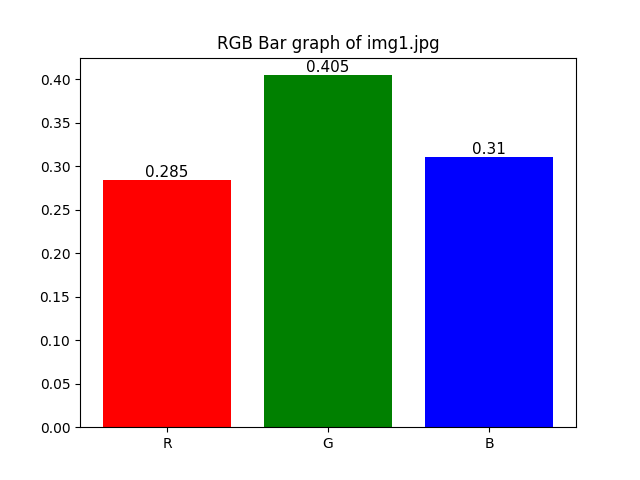
\includegraphics[width=0.5\textwidth]{img1.jpg_RGB_Bar.png}
	
}
\subfigure[灰度直方图]{
	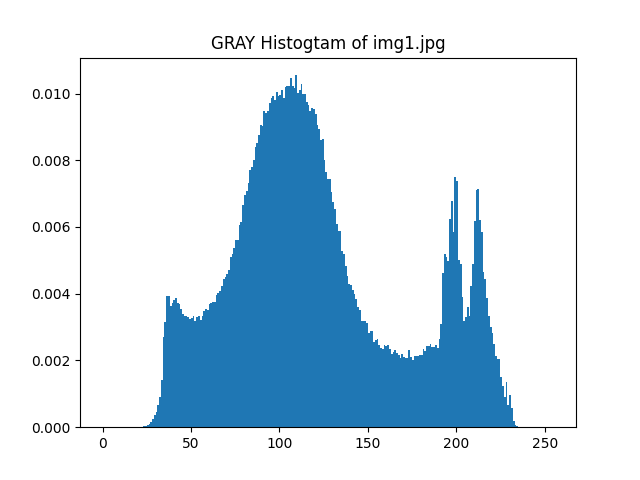
\includegraphics[width=0.5\textwidth]{img1.jpg_GRAY_Hist.png}
	
}	
\subfigure[梯度直方图]{
	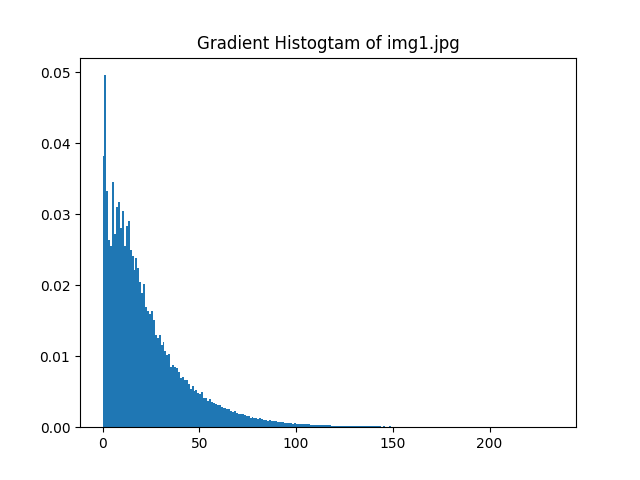
\includegraphics[width=0.5\textwidth]{img1.jpg_GRAD_Hist.png}
	\centering
}
\subfigure[原图]{
	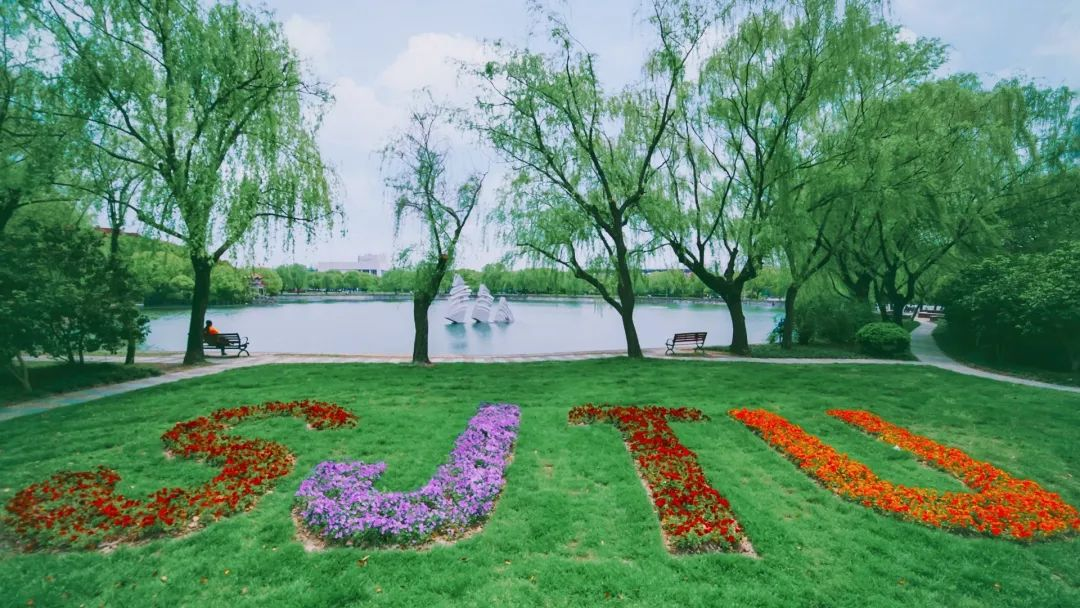
\includegraphics[width=0.5\textwidth]{img1.jpg}
	\centering
}
	\caption{img1.jpg}
	\centering
\end{figure}


\begin{figure}[H]
\subfigure[颜色直方图]{
	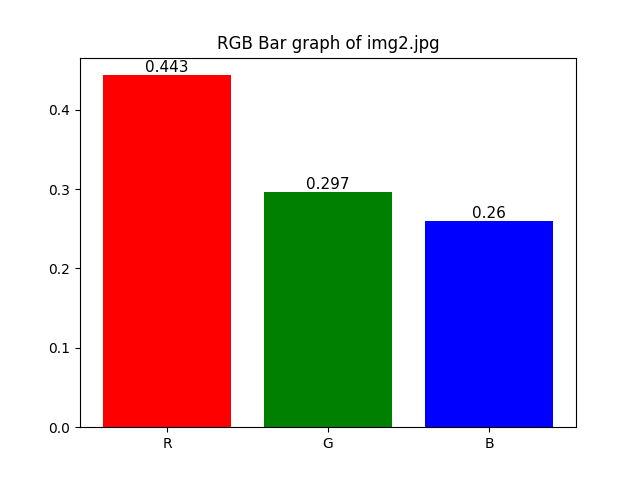
\includegraphics[width=0.5\textwidth]{img2.jpg_RGB_Bar.png}
	
}
\subfigure[灰度直方图]{
	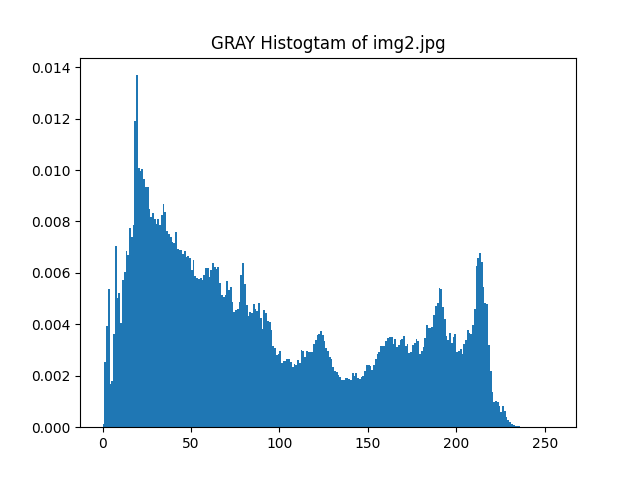
\includegraphics[width=0.5\textwidth]{img2.jpg_GRAY_Hist.png}
	
}	
\subfigure[梯度直方图]{
	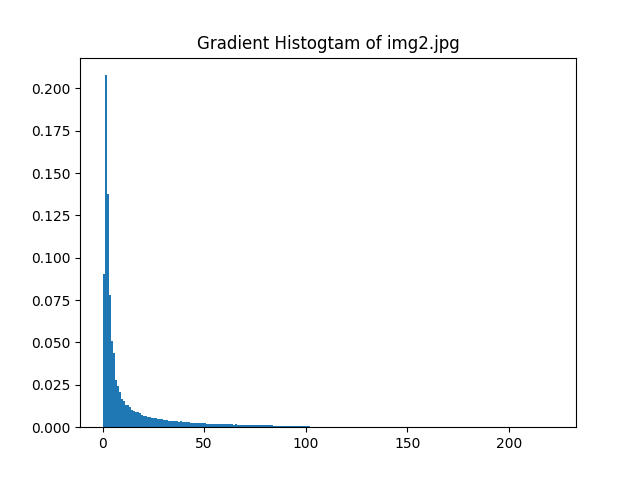
\includegraphics[width=0.5\textwidth]{img2.jpg_GRAD_Hist.png}
	\centering
}
\subfigure[原图]{
	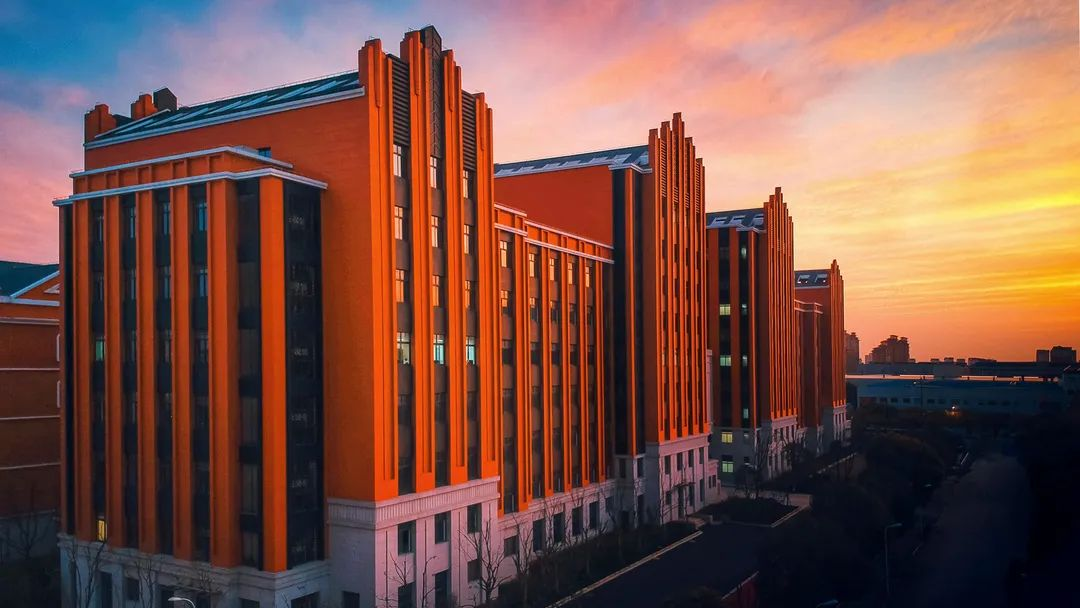
\includegraphics[width=0.5\textwidth]{img2.jpg}
	\centering
}
	\caption{img2.jpg}
	\centering
\end{figure}

\begin{figure}[H]
\subfigure[颜色直方图]{
	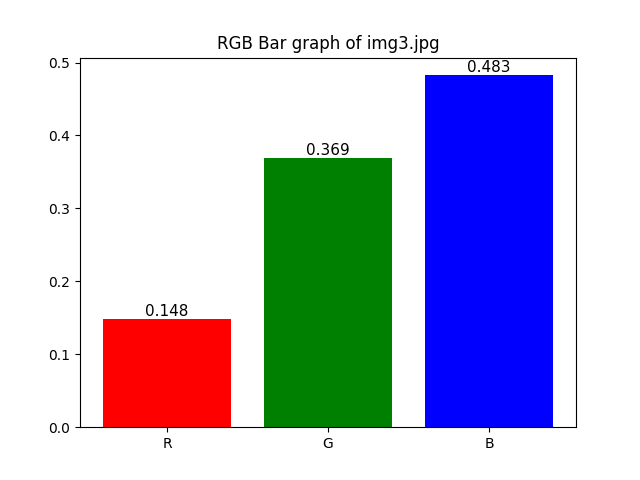
\includegraphics[width=0.5\textwidth]{img3.jpg_RGB_Bar.png}
	
}
\subfigure[灰度直方图]{
	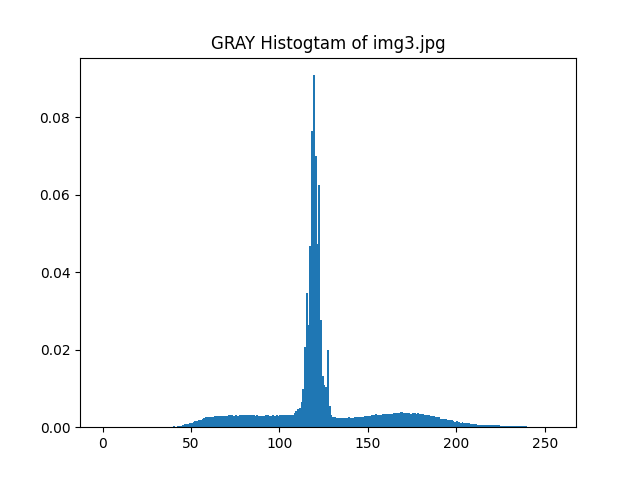
\includegraphics[width=0.5\textwidth]{img3.jpg_GRAY_Hist.png}
	
}	
\subfigure[梯度直方图]{
	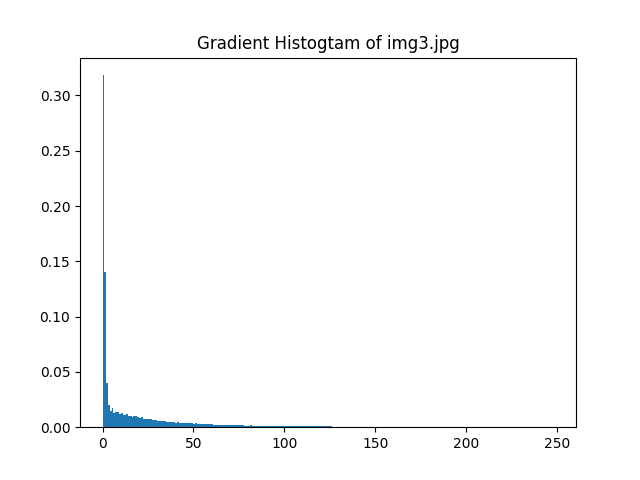
\includegraphics[width=0.5\textwidth]{img3.jpg_GRAD_Hist.png}
	\centering
}
\subfigure[原图]{
	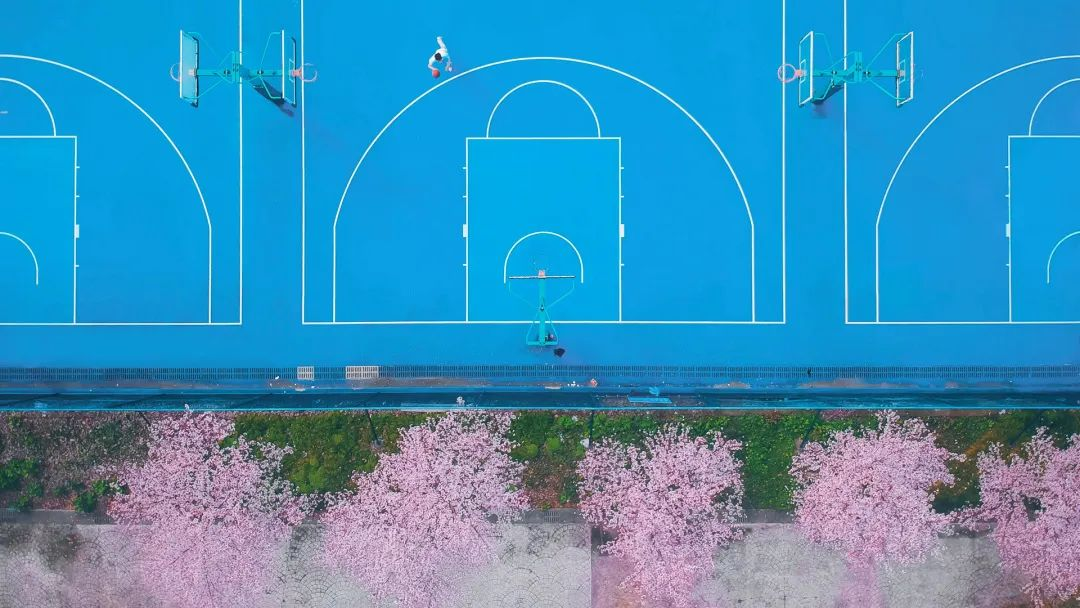
\includegraphics[width=0.5\textwidth]{img3.jpg}
	\centering
}
	\caption{img3.jpg}
	\centering
\end{figure}
\section{分析与思考}
\begin{itemize}
\item 颜色直方图反映了图片中RGB三种颜色的多少,比如B比较高的人眼看起来整张图蓝色偏多。
\item 灰度直方图峰值位置体现了图片的明暗,分布集中程度则体现为对比度。
\item 梯度(强度)直方图体现了图片纹理简单或复杂。纹理复杂的图片分布比较均匀,反之分布集中在梯度比较小的地方。
\item 图片梯度计算由于有平方、开根号操作,运行效率较低,一张图要跑几秒钟;
\item 画图片直方图一定要对数据进行归一化操作,以消除图片大小尺寸的影响。
\end{itemize}

\end{document}

